\documentclass{article}
\usepackage[utf8]{inputenc}
\usepackage{graphicx}
\usepackage[margin=35mm]{geometry}


\title{Automatically defend from DoS and DDoS traffic flood attacks}
\author{Yinon Cohen and Maor Shabtay }
\date{November 2017}

\begin{document}
\maketitle

\hfill \break DoS and DDoS attacks are attempts to exhaust server side assets, and designed to prevent client-to-server communication (denial of service). These attacks aim to both public and private sectors, and occur more and more frequently. In addition, lately the massive DDoS attacks are performing 100 Gigabits per second, and being more common than ever. These attacks are sowing fear among organizations and private server owners.

\hfill \break Our project deals with understanding and examining DoS and DDoS attacks, and what are the solutions for them. In particularly, we will discuss and handle with traffic flood attacks on web servers, and will try to develop our own software or algorithm to block or to give any immediately pragmatic solution.

\hfill \break Our main goal is to develop an automatic system that would identify and analyze a traffic flood attack, defend the server from it, and in need - will block any IP or sub-net which the flood comes from. Our system should run on a CDN instead of on the server in order to save the server’s performances providing service
\hfill \break \hfill \break
    \begin{center}
        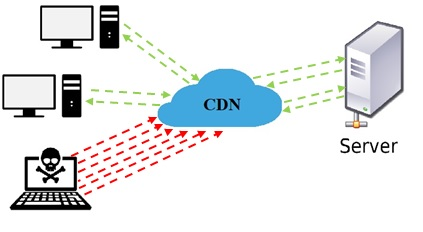
\includegraphics{pi}
    \end{center}
 \hfill \break Advisor: Dr. Amit Dvir
 \hfill \break Students: 
 \hfill \break Yinon Cohen 203526991
 \hfill \break Maor Shabtay 305036162


\end{document}
